\documentclass[border=10pt]{standalone}
\usepackage{tikz}
\usetikzlibrary{arrows.meta, shapes, calc}

\begin{document}
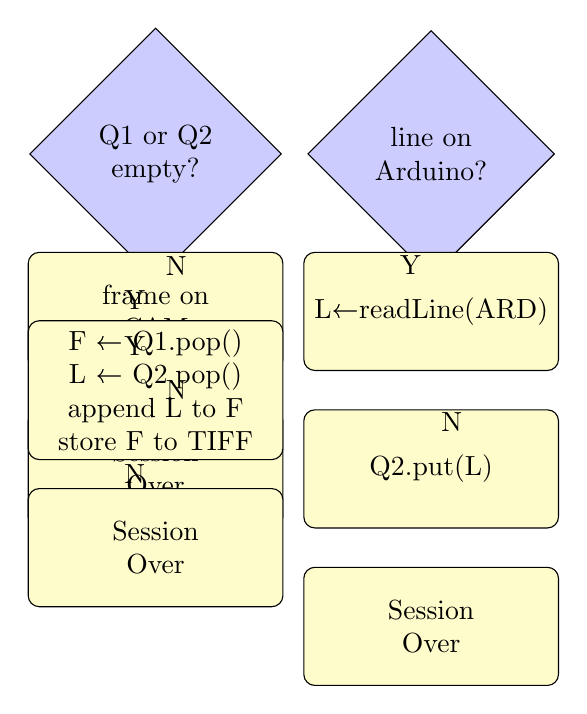
\begin{tikzpicture}[
  node distance = 1.5cm,
  auto,
  block/.style = {rectangle, rounded corners, draw, fill=yellow!20, text width=3cm, text centered, minimum height=1.5cm},
  decision/.style = {diamond, draw, fill=blue!20, text width=2cm, text centered, minimum height=1cm},
  session/.style = {rectangle, rounded corners, draw, fill=green!20, text width=2cm, text centered, minimum height=1cm},
  arrow/.style = {thick, -Latex}
]

  % Nodes
  \node [decision] (q1q2empty) {Q1 or Q2\\empty?};
  \node [block, below of=q1q2empty, yshift=-0.5cm] (frameoncam) {frame on\\CAM};
  \node [block, below of=frameoncam, yshift=-0.5cm] (session1) {Session\\Over};
  \node [decision, right of=q1q2empty, xshift=2cm] (lineonarduino) {line on\\Arduino?};
  \node [block, below of=lineonarduino, yshift=-0.5cm] (readlineard) {L←readLine(ARD)};
  \node [block, below of=readlineard, yshift=-0.5cm] (q2putl) {Q2.put(L)};
  \node [block, below of=q2putl, yshift=-0.5cm] (session2) {Session\\Over};
  \node [block, below of=q1q2empty, yshift=-1.5cm] (fappend) {F ← Q1.pop()\\L ← Q2.pop()\\append L to F\\store F to TIFF};
  \node [block, below of=fappend, yshift=-0.5cm] (session3) {Session\\Over};

  % Arrows
  \path [arrow] (q1q2empty) -- node[anchor=east] {Y} (fappend);
  \path [arrow] (q1q2empty) -- node[anchor=west] {N} (frameoncam);
  \path [arrow] (frameoncam) -- node[anchor=east] {Y} (fappend);
  \path [arrow] (frameoncam) -- node[anchor=west] {N} (session1);
  \path [arrow] (lineonarduino) -- node[anchor=east] {Y} (readlineard);
  \path [arrow] (lineonarduino) -- node[anchor=west] {N} (session2);
  \path [arrow] (readlineard) -- (q2putl);
  \path [arrow] (q2putl) -- (session2);
  \path [arrow] (fappend) -- node[anchor=east] {N} (session3);
  \path [arrow] (session1) -- (session3);
  \path [arrow] (session2) -- (session3);

\end{tikzpicture}
\end{document}